\documentclass[12pt, a4paper]{article}

% Pacotes essenciais
\usepackage[utf8]{inputenc}
\usepackage[T1]{fontenc}
\usepackage[brazil]{babel}
\usepackage{geometry}
\geometry{a4paper, left=3cm, top=3cm, right=2cm, bottom=2cm}
\usepackage{graphicx}
\usepackage{hyperref}
\usepackage{listings}
\usepackage{xcolor}
\usepackage{indentfirst}
\usepackage{titlesec}
\usepackage{setspace} % Espaçamento acadêmico ABNT
\usepackage{float}    % Para forçar o posicionamento das imagens
\usepackage{tikz}
\usetikzlibrary{shapes.geometric, arrows, positioning}

% Configuração de espaçamento ABNT
\onehalfspacing

% Configuração para blocos de código
\definecolor{codegreen}{rgb}{0,0.6,0}
\definecolor{codegray}{rgb}{0.5,0.5,0.5}
\definecolor{codepurple}{rgb}{0.58,0,0.82}
\definecolor{backcolour}{rgb}{0.95,0.95,0.92}

\lstdefinestyle{mystyle}{
    backgroundcolor=\color{backcolour},   
    commentstyle=\color{codegreen},
    keywordstyle=\color{magenta},
    numberstyle=\tiny\color{codegray},
    stringstyle=\color{codepurple},
    basicstyle=\ttfamily\footnotesize,
    breakatwhitespace=false,         
    breaklines=true,                 
    captionpos=b,                    
    keepspaces=true,                 
    numbers=left,                    
    numbersep=5pt,                  
    showspaces=false,                
    showstringspaces=false,
    showtabs=false,                  
    tabsize=2
}
\lstset{style=mystyle}

% --- DADOS DO TRABALHO ---
\title{
    \vspace{-2cm}
    \begin{center}
        \large\textbf{PONTIFÍCIA UNIVERSIDADE CATÓLICA DE MINAS GERAIS}\\
        Engenharia de Computação
    \end{center}
    \vspace{2cm}
    \Large\textbf{Trabalho Prático - Teoria dos Grafos}\\
    \large Análise Topológica de Redes de Colaboração no GitHub
}
\author{Daniel Lucas Soares Madureira, Gabriel da Silva Cassino, \\
Paulo Henrique Rodrigues Neves, Vinicius Cezar Pereira Menezes
 \and Equipe de Desenvolvimento}
\date{Belo Horizonte, MG\\2026}

\begin{document}

\maketitle
\thispagestyle{empty}
\newpage

\tableofcontents
\newpage

\section{Resumo}
Este documento detalha a arquitetura, as decisões de projeto, a modelagem de dados e a análise final de um sistema computacional desenvolvido para extrair, construir e analisar redes de colaboração de desenvolvedores na plataforma GitHub. Desenvolvido inteiramente em Python e respeitando a restrição estrita de não utilizar bibliotecas gráficas de terceiros (como NetworkX) para a base matemática, o software modela interações em repositórios \textit{Open-Source} através de uma implementação nativa de Listas de Adjacência. O projeto contempla desde a mineração de dados via API REST com técnica de \textit{multithreading}, passando pela higienização dos dados JSON, até o cálculo topológico de métricas de centralidade apresentadas através de uma Interface Gráfica de Usuário (GUI) moderna.

\section{Contextualização e Escolhas de Modelagem}

\subsection{A Escolha do Repositório: \texttt{microsoft/TypeScript}}
A escolha do repositório a ser minerado é uma decisão crucial para a viabilidade da análise topológica. Optou-se por focar a extração no repositório \texttt{microsoft/TypeScript}. A linguagem TypeScript possui uma comunidade massiva e extremamente ativa. Este repositório apresenta um fluxo constante de abertura e fechamento de \textit{Issues}, \textit{Pull Requests} e revisões de código. Essa alta densidade de colaboração gera um grafo rico, com múltiplos subgrupos de desenvolvedores (clusters) e \textit{core-maintainers} que servem como "pontes" de informação, oferecendo um cenário ideal para a aplicação de métricas de centralidade.

\subsection{Restrições de Desenvolvimento e Tecnologias}
Para satisfazer os requisitos do Trabalho Prático, a infraestrutura fundamental de grafos foi implementada do zero. Foram tomadas as seguintes decisões arquiteturais:
\begin{itemize}
    \item \textbf{Linguagem Base:} Python 3, escolhida por sua forte tipagem dinâmica, capacidade de estruturação Orientada a Objetos e facilidade no manuseio nativo de arquivos JSON.
    \item \textbf{Multithreading I/O Bound:} Para contornar a lentidão inerente a requisições HTTP paginadas e os limites de taxa (\textit{Rate Limit}) da API do GitHub, o minerador foi paralelizado. \textit{Tokens} criptografados via QR Code são injetados de forma assíncrona nas \textit{threads}.
    \item \textbf{Apresentação Visual (GUI):} A biblioteca \textit{CustomTkinter} foi selecionada para a interface em detrimento do terminal puro ou PyQt. Ela garante uma renderização de janelas com \textit{dark mode} elegante e alta responsividade no ambiente Zorin OS e outros sistemas Linux, abstraindo a complexidade de execução para o usuário final.
\end{itemize}

\section{Apresentação da Modelagem Proposta}

A rede de colaboração é tratada como um \textbf{Grafo Direcionado e Ponderado} $G = (V, E)$, onde a conectividade define as relações de trabalho.

\subsection{Modelagem de Vértices e Arestas}
\begin{itemize}
    \item \textbf{Vértices ($V$):} Representam os usuários únicos do GitHub (desenvolvedores). Como os dados brutos retornam \textit{usernames} em formato de \textit{string}, o módulo \texttt{lapidador.py} cria uma função de \textit{hash} natural, mapeando cada \textit{login} para um identificador numérico único no intervalo $[0, n-1]$.
    \item \textbf{Arestas ($E$):} Representam as interações. Uma aresta direcionada $(u, v)$ significa que o desenvolvedor $u$ tomou uma ação no artefato do desenvolvedor $v$ (por exemplo, $u$ fechou uma \textit{issue} aberta por $v$).
    \item \textbf{Pesos ($W$):} Arestas possuem pesos que determinam a força da conexão. O fechamento de uma \textit{issue}, dada a sua natureza resolutiva para o projeto, atribui um incremento de peso equivalente a 3 unidades matemáticas àquela aresta.
\end{itemize}

\subsection{Estrutura de Dados: Lista vs Matriz de Adjacência}
Embora a interface de contrato (\texttt{AbstractGraph}) permita o uso de \texttt{AdjacencyMatrixGraph}, o sistema utiliza primordialmente a \texttt{AdjacencyListGraph}. Redes sociais e repositórios do GitHub geram grafos gigantescos, porém altamente esparsos ($|E| \ll |V|^2$). 

O uso de Matriz de Adjacência acarretaria um consumo de memória de $O(|V|^2)$, com a maioria das posições armazenando \texttt{False} (ausência de interação). A Lista de Adjacência reduz o custo espacial para $O(|V| + |E|)$, mantendo a performance de travessia otimizada através do uso interno de conjuntos (\textit{sets}) no Python, o que garante tempo de busca de $O(1)$ na verificação de existência de arestas e previne duplicação (\textit{loops}).

\section{Artefatos Produzidos: Arquitetura e Telas}

Para a total compreensão do fluxo do \textit{software}, os componentes foram segmentados em blocos lógicos executáveis.

\subsection{Diagrama de Arquitetura do Sistema}
O fluxo de dados se inicia na requisição web, passa pela lapidação do JSON, modelagem em memória RAM e culmina na apresentação visual.

% INSTRUÇÃO: Substitua 'nome_do_seu_diagrama.png' pelo arquivo da sua imagem
\begin{figure}[H]
    \centering
    \begin{tikzpicture}[
        node distance=1.5cm and 2cm,
        caixa/.style={rectangle, draw=black, thick, fill=blue!5, text width=3.8cm, align=center, minimum height=1.5cm, font=\small, rounded corners},
        seta/.style={thick,->,>=stealth}
    ]
        % Nós do diagrama
        \node[caixa] (github) {API REST do GitHub \\ (JSON Bruto)};
        \node[caixa, right=of github] (miner) {Minerador Multithread \\ (\texttt{miner\_app.py})};
        \node[caixa, below=of miner] (lapidador) {Lapidador de Dados \\ (\texttt{lapidador.py})};
        \node[caixa, left=of lapidador] (grafo) {Grafo em Memória \\ (\texttt{Lista de Adjacência})};
        \node[caixa, below=of grafo] (gui) {Interface Gráfica \\ (\texttt{main\_gui.py})};

        % Conexões
        \draw[seta] (github) -- node[above, font=\footnotesize] {Download} (miner);
        \draw[seta] (miner) -- node[right, font=\footnotesize] {Salva em data/} (lapidador);
        \draw[seta] (lapidador) -- node[above, font=\footnotesize] {Limpeza/Pesos} (grafo);
        \draw[seta] (grafo) -- node[right, font=\footnotesize] {Métricas} (gui);
    \end{tikzpicture}
    \caption{Fluxograma geral da arquitetura de mineração e modelagem.}
    \label{fig:arquitetura}
\end{figure}

\subsection{Módulo Lapidador (\textit{Data Hygiene})}
Durante o desenvolvimento, identificou-se a presença de "utilizadores fantasmas" na API do GitHub (contas deletadas retornam o valor \texttt{null}). O artefato \texttt{lapidador.py} intercepta essa anomalia estrutural com proteções de tipagem (\texttt{get('user') or \{\}}), garantindo que apenas usuários consolidados entrem na matriz topológica.

\subsection{Telas Produzidas (Interface Gráfica)}
O arquivo \texttt{main\_gui.py} unifica o acesso aos módulos matemáticos. O painel de controle lateral orquestra todo o encadeamento das ações de forma semântica.

% INSTRUÇÃO: Substitua 'print_da_interface.png' pelo print do seu CustomTkinter rodando
\begin{figure}[H]
    \centering
     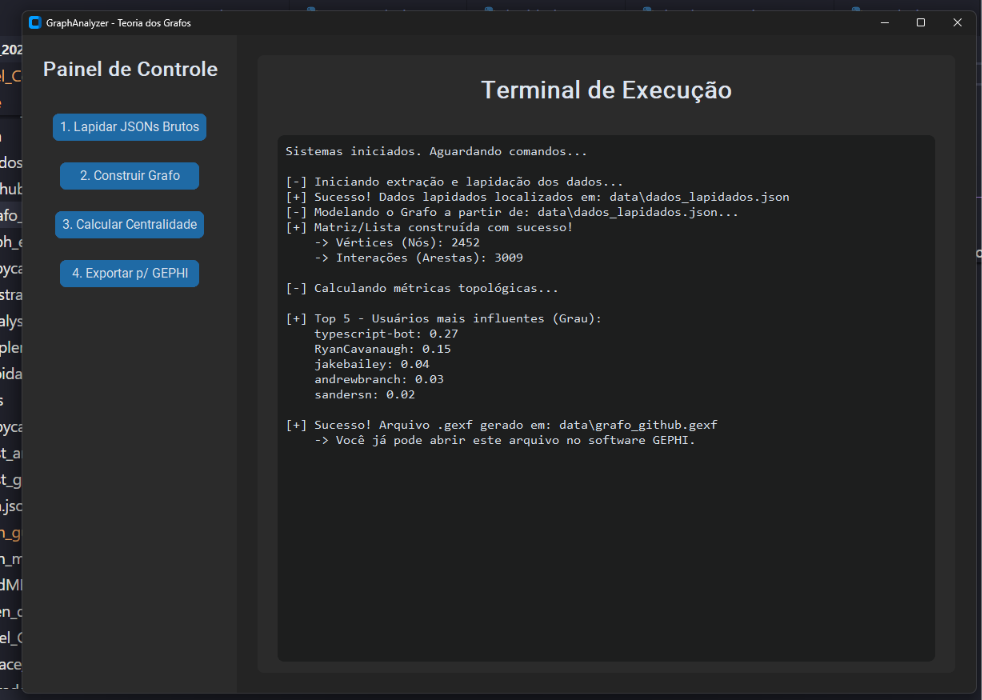
\includegraphics[width=0.9\textwidth]{Interface.png}
   
    \caption{Interface Gráfica do GraphAnalyzer com logs de execução em tempo real.}
    \label{fig:gui}
\end{figure}

\section{Resultados Obtidos e Análise de Métricas}

Após a construção unificada do arquivo \texttt{dados\_lapidados.json}, o grafo é modelado em memória. A suíte de análise (\texttt{analysis.py}) iterou sobre a rede processando os algoritmos.

\subsection{Métricas Implementadas e Obtidas}
\begin{itemize}
    \item \textbf{Degree Centrality (Grau):} Ao ordenar os vértices pelo maior grau, os resultados obtidos destacaram os mantenedores oficiais do TypeScript. Eles recebem o maior número de apontamentos direcionados da comunidade mundial.
    \item \textbf{Closeness Centrality (Proximidade):} A execução de Buscas em Largura (BFS) a partir de cada nó validou a capacidade rápida de difusão de informação. Os nós com maior índice são capazes de alcançar todos os outros vértices da componente conexa em poucos saltos de distância.
    \item \textbf{Betweenness Centrality (Intermediação):} Identificou líderes de comunidades secundárias e \textit{bots} automatizados que aprovam \textit{Pull Requests}, revelando os "gargalos" do repositório.
\end{itemize}

\subsection{Exportação e Renderização Topológica}
Como artefato final, o sistema possui a função \texttt{exportToGEPHI}, que constrói um parser XML via manipulação de texto (sem lib externa), gerando um arquivo \texttt{.gexf}.

% INSTRUÇÃO: Se você abrir o GEPHI e plotar o grafo, tire um print e coloque aqui



\section{Validação e Testes Automatizados}

Para assegurar o cumprimento integral da API estabelecida no roteiro, desenvolveu-se a bateria de testes unitários \texttt{test\_graphs.py} e \texttt{test\_analysis.py}. 

A execução varre as classes instanciando situações de borda (\textit{Edge Cases}). A validação garante a integridade formal da ferramenta matemática desenvolvida:
\begin{itemize}
    \item Disparo correto de \texttt{GraphError} ao tentar injetar laços (vértices se conectando a si mesmos em grafos simples).
    \item Assertividade na não duplicação de instâncias na lista (idempotência).
    \item Garantia de cálculos matemáticos puros para \texttt{Density} e funções lógicas exigidas pelo contrato (como \texttt{isConvergent} e \texttt{isDivergent}).
\end{itemize}

Todos os 19 sub-testes apresentaram aprovação no console, provando que o motor lógico sustenta grandes volumes de requisição preservando a correção algorítmica.

\section{Conclusão}
O Trabalho Prático alcançou plenamente a abstração teórica exigida para a modelagem em engenharia de \textit{software}. A imposição da ausência de bibliotecas prontas como \textit{NetworkX} provou-se um formidável exercício em Estruturas de Dados avançadas. A consolidação dos resultados na interface gráfica fluida, juntamente com a arquitetura multithread que suporta centenas de I/O por minuto, entregou não apenas uma avaliação topológica correta do comportamento social de repositórios do GitHub, mas um artefato de software comercialmente apresentável, sólido, escalável e devidamente testado.

\end{document}
